\section{Raumerkennung}

Die Raumerkennung ist der wichtigste Aspekt unserer Anwendung.
Die zugrundeliegende Idee ist, dass stationäre Beacons in den
relevanten Räumen platziert werden. Anschließend werden diese
Räume einmalig vermessen, um ein Modell zur Erkennung der
Räume zu erstellen.
Dabei ist zu beachten, dass wir im Gegensatz zu anderen Projekten
im Bereich In-Door-Lokalisation keine Informationen über die
Räume oder die Position der Beacons besitzen. Aus diesem Grund
beschränken wir die Genauigkeit der Positionsbestimmung auf
Raumebene.

Im Folgenden wird beschrieben, wie wir die Messung der Beacons
durchgeführt haben. 

\subsection{Idee}

Wie wollen wir die Raumlösung umsetzen?
- Verwendung von stationären Beacons
- Vermessen von Räumen
- Keine Information über Räume (Karten)
- Keine Information, wo sich die Beacons befinden

\subsection{Messung}

Was ist eine Messung?
- Vektor von (normalisierten) RSSI-Werten
Wie haben wir die Messung durchgeführt?
- RSSI-Werte von Beacons gemessen
- Problem 1: Werte kommen ca. jede Sekunde aber zu unterschiedlichen Zeitpunkten
  Was bedeutet gleichzeitige Messung von mehreren Beacons?
- Problem 2: Was tun, wenn ein Beacon nur kurz nicht gemessen wurde und deshalb
  in der letzten Sekunde nicht gemessen wurde?
- Lösung: Modell zur Messung mehrere Beacons und Definition des Begriffs der
  pseudogleichzeitigen Messung.

\subsection{Machbarkeitsanalyse}

Analyse: Ist es überhaupt möglich Räume anhand von Messwerten zu unterscheiden?
Erste Messung:
- Messungen in Form von Mittelwert + Stddev vorstellen
- Messungen in Grafikform vorstellen
- Ergebnis: Räume sind unterscheidbar

\subsection{Lösungsansatz}

Gezeigt: Es ist machbar. Jetzt klären wie?
Zwei Probleme:
- Problem 1: Um eine Messung einem Raum zuzuordnen, brauchen wir ein Vorhersagemodell,
  das aus dem Messvektor den wahrscheinlichsten Raum berechnet.
- Problem 2: Eine Messung allein reicht nicht aus, um eine korrekte Aussage über
  den aktuellen Raum zu machen. Wir brauchen zusätzlich ein Zuordnungsmodell,
  das aus mehreren aufeinanderfolgenden Vorhersagen den aktuellen Raum sicher
  bestimmt.
  
\subsection{Implementierung}

Vorhersagemodell:
- Webservice in Python
- Verwendung von TensorFlow
- Machine-Learning für Bestimmen der Parameter
Zuordnungsmodell:
- Mehrfache Messung + Vorhersage
- LimitedQueue mit alten Vorhersagen
- Mehrheit in dieser Queue bestimmt, welcher Raum zugeordnet wird
- Effekt: Hysterese

\subsection{Erstes Szenario}

Da uns zu Beginn des Projekts nur zwei G-Tags zur Verfügung standen, betrachten
wir zunächst ein vereinfachtes Szenario:
\begin{itemize}
	\item Es gibt zwei Räume: Küche, Flur
	\item In jedem Raum ist ein G-Tag platziert
\end{itemize}

\subsubsection{Messung}

Mithilfe eines rudimentären Bluetooth-Scanners vermessen wir die einzelnen Räume.
Dabei werden mehrere Scans durchgeführt. Ein Scan enthält die Signalstärke 
jedes Beacons in der Einheit RSSI (Received Signal Strength Indication).
Die wahrgenommene Signalstärke hängt von vielen Faktoren ab:
\begin{itemize}
	\item Wie stark sendet der Beacon?
	\item Wie gut ist die Antenne im Smartphone bzw. der Smartwatch?
	\item Wie weit sind Sender und Empfänger entfernt?
	\item Welche Störungen (Reflektionen, Abdeckungen) gibt es?
	\item Wie hat der Hersteller des Empfängers die Übersetzung von Feldstärke in RSSI-Wert implementiert?
\end{itemize}
Eine direkte Positionsbestimmung über z.B. Triangulation ist also schwierig.
In unserem Problem kommt noch dazu, dass wir über keine Karte der Räume
verfügen.

Die Signalstärken der Beacons werden ca. jede Sekunde gemessen ($\delta t_m \approx 1s$).
Die Messung der einzelnen Beacons erfolgt allerdings zu unterschiedlichen Zeiten,
weshalb wir ein Zeitfenster von $\Delta t_g = 2s$ in dem Messungen unterschiedlicher
Beacons als gleichzeitig angesehen werden. Dadurch werden Beacons, die in der letzten Sekunde aus irgendeinem Grund nicht gemessen werden konnten, nicht direkt als nicht vorhanden eingestuft.
Erst wenn ein Beacon in zwei aufeinanderfolgenden Messungen nicht registriert wurde, wird dessen Signalstärke als nicht vorhanden angesehen.

\subsubsection{Ergebnis}

Als erstes Betrachten wir den Minimal-, Maximal, Mittelwert und Standardabweichung für jeden
Beacon in jedem Raum. Diese bestimmen wir per SQL aus der SQLite-Datenbank der Messwerte.

\begin{tabular}{|c|c|c|c|c|c|}
	\hline \textbf{Raum} & \textbf{Tag} & \textbf{min(RSSI)} & \textbf{max(RSSI)} & \textbf{avg(RSSI)} & \textbf{stddev(RSSI)} \\ 
	\hline Küche  & 7C:2F:80:8D:E2:3B & -82 & -40 & -60,36 & 12,46 \\ 
	\hline Küche & 7C:2F:80:8D:E2:45 & -88 & -69 & -78,61 & 9,29 \\ 
	\hline Flur & 7C:2F:80:8D:E2:3B & -94 & -64 & -78,67 & 9,95 \\ 
	\hline Flur & 7C:2F:80:8D:E2:45 & -83 & -49 & -67,38 & 7,53 \\ 
	\hline 
\end{tabular}

\vspace{0.4cm}
Wie erwartet, gibt es relativ große Schwankungen bei den einzelnen Messwerten.
Allerdings lässt sich an den Durchsnittswerten ablesen, dass die beiden Räume
prinzipiell auseinander gehalten werden können.

\subsubsection{Visualisierung}
Da man sich unter einer Liste von Messwerten häufig wenig vorstellen kann,
wollen wir zunächst die Messung in einer Grafik visualisieren.

\begin{figure}[tbh]
\centering
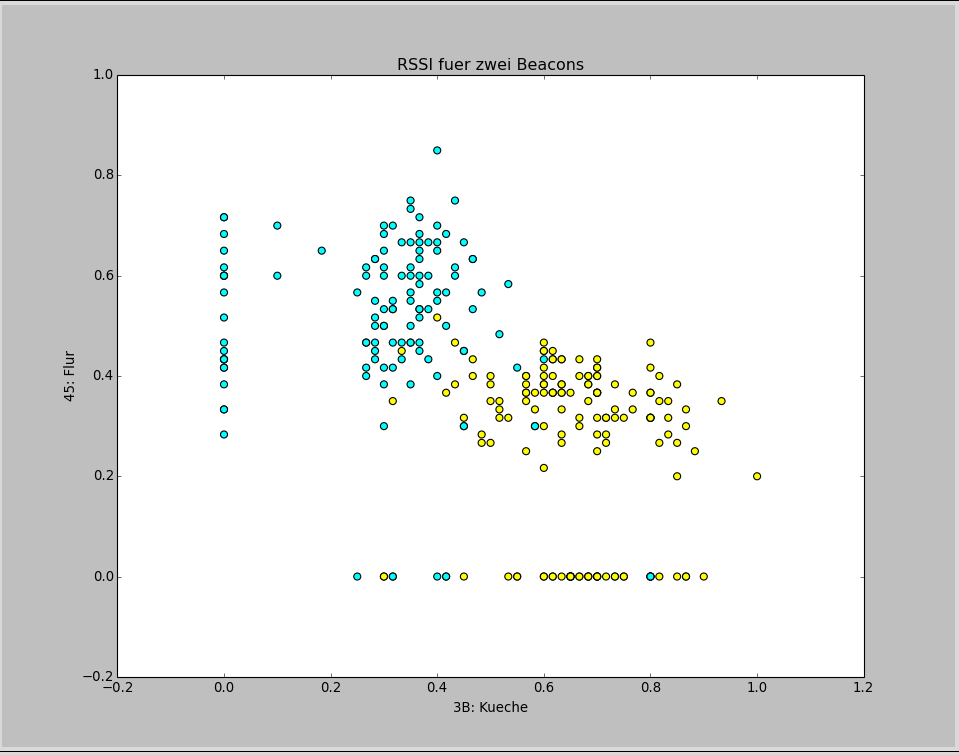
\includegraphics[width=1.0\linewidth]{Bilder/Messungen/KuecheFlur_1}
\caption{Messung von Küche und Flur mit zwei Beacons}
\label{fig:KuecheFlur_1}
\end{figure}
